\documentclass[journal,twocolumn]{IEEEtran}

% --- Core Packages ---
\usepackage{cite}
\usepackage{graphicx}
\usepackage{amsmath,amssymb,amsfonts}
\usepackage{algorithmic}
\usepackage{url}
\usepackage{hyperref}
\usepackage{titlesec}
\usepackage[font=small,labelfont=bf]{caption}
\usepackage{tabularx}
\usepackage{booktabs}
\graphicspath{{figures/}{organoid_rl/experiments/results/paper_figures/}{./}}

% --- Spacing Fixes ---
\addtolength{\thinmuskip}{1mu}
\setlength{\parskip}{0.3em}

% --- Heading Customization ---
\titleformat{\section}{\large\bfseries}{\thesection.}{1em}{}
\titleformat{\subsection}{\normalsize\bfseries}{\thesubsection.}{1em}{}
\titleformat{\subsubsection}{\normalsize\bfseries\itshape}{\thesubsubsection.}{1em}{}
\titleformat{\subparagraph}[runin]{\normalfont\normalsize\bfseries}{\thesubparagraph}{1em}{}

% ---------------------------------------------------------------
\begin{document}

\title{OrganoidEnv: A Stabilized Reinforcement Learning Environment for
Training Biologically Constrained Spiking Neural Networks via
Sensory--Motor Mapping}

\author{Vansh~Sharma and Dr.~Seema~Malik%
\thanks{V.~Sharma and Dr.~S.~Malik are with the School of Engineering
\& Technology, Vivekananda Institute of Professional Studies --
Technical Campus, AU-Block (Outer Ring Road), Pitampura,
Delhi~110034, India (e-mail: \texttt{02717711724\_IIOT@vipstc.edu};
\texttt{simadahiva@gmail.com}).
Word count (body, excluding abstract and references):
$\approx$\,5{,}200 words.}}

\markboth{Journal of \LaTeX\ Class Files,~Vol.~14, No.~8,
          August~2026}{Sharma \& Malik: OrganoidEnv}

\maketitle

% ---------------------------------------------------------------
\begin{abstract}
\textbf{Background:} Integrating biologically realistic spiking neural
networks (SNNs) with reinforcement learning (RL) is hindered by spike
non-differentiability and recurrent instability.  This study introduces
OrganoidEnv, a Gymnasium-compatible environment designed to train a
500-neuron metabolic-Izhikevich network as a controllable \emph{in
silico} ``organoid.''

\textbf{Methods:} Unlike surrogate-gradient methods, OrganoidEnv uses
an outer Dueling Double Deep Q-Network (D3QN) that interacts with the
SNN via sensory--motor current stimulation.  Stability is maintained
through a Global Activity Regulator (GAR), homeostatic inhibitory
scaling, and a dopamine-inspired dual-trace eligibility rule for local
plasticity.

\textbf{Results:} Evaluated on a 2D navigation task across independent biological random seeds ($N=3$, 200 episodes each), the system achieved a $71.3\% \pm 40.1\%$ success rate in Stage~1 basic navigation (with top seeds reaching $95.0\%$ and $94.0\%$) and $62.0\% \pm 38.4\%$ during obstacle curriculum adaptation (overall multi-seed completion: $66.7\% \pm 39.2\%$, with top seeds reaching $92.0\%$ and $86.5\%$). Multi-seed ablation studies confirmed that removing the Global Activity Regulator (GAR) causes severe dynamical instability (reward variance $\pm 93.70$), while omitting Sparse Distributed Memory (SDM) causes complete sensory collapse ($3.7\%$ success). The SNN maintained a biologically realistic average firing rate of 8.5\,Hz.

\textbf{Conclusion:} These results demonstrate that an external RL agent can effectively ``tame'' and train a biologically constrained SNN. OrganoidEnv is released as an open-source, Gymnasium-compatible testbed---the first to combine metabolic-Izhikevich neurons, homeostatic stabilizers, and dual-trace plasticity in a single reproducible package---providing the neuromorphic computing community with a standardized benchmark for biologically constrained RL--SNN co-training.
\end{abstract}

\begin{IEEEkeywords}
Spiking Neural Networks, Reinforcement Learning, Neuromorphic
Computing, Organoid Intelligence, Sensory--Motor Mapping, Synaptic
Plasticity
\end{IEEEkeywords}

% ---------------------------------------------------------------
\section*{Plain Language Summary}

This study introduces OrganoidEnv, a digital simulation that mimics
the learning process of biological brain cells.  Using an artificial
intelligence ``coach'' to guide a network of simulated neurons through
current-based stimulation, we show that these biologically constrained
models can learn to navigate complex paths and avoid obstacles.  The
system preserves the key properties of real neural tissue---metabolic
fatigue, local synaptic plasticity, and homeostatic regulation---while
remaining fully reproducible and controllable in software.  OrganoidEnv
provides a bridge between artificial intelligence and biological brain
research and offers a testbed for future neuromorphic and
organoid-inspired computing experiments.

% ===============================================================
\section{Introduction}
% ===============================================================

\IEEEPARstart{S}{piking} neural networks (SNNs) are a central
abstraction for neuromorphic computation due to their event-driven
communication, temporal coding, and close correspondence to biological
neurons and synapses \cite{Izhikevich2003simple,NeuromorphicReview2019}.
In contrast, artificial neural networks (ANNs) trained with
backpropagation deliver state-of-the-art performance across domains
but typically ignore biophysical constraints, such as sparse firing,
local plasticity, and metabolic limits \cite{Mnih2015human}.
Bridging the gap between high-performing deep RL and biologically
grounded SNNs remains an open challenge.

Classical spike-timing-dependent plasticity (STDP) and
reward-modulated STDP (R-STDP) provide local learning rules but
struggle with temporal credit assignment in delayed-reward tasks,
especially in recurrent networks
\cite{Florian2007rstdp,FarriesFairhall2007}.  Surrogate-gradient
methods and e-prop approximate backpropagation through time for
spiking systems \cite{Bellec2018l2l,DirectTrainingSNN2024}, yet they
often sacrifice biological plausibility by relying on continuous
relaxations and storing long histories of membrane state.

In parallel, recent work on \emph{organoid intelligence} (OI) has
proposed the combination of living brain organoids with machine
interfaces to create hybrid biocomputing systems
\cite{Smirnova2023OI,Hartung2023OIworkshop}.  Although \emph{in
vitro} organoids provide biological realism, they are expensive,
fragile, and experimentally constrained.  There is a need for
\emph{in silico} organoid analogues that capture the key principles
of organoid learning and plasticity while remaining reproducible and
controllable.

This study proposes \emph{OrganoidEnv}, a stabilized RL environment
that treats a biologically constrained SNN as an \emph{actor embedded
in an environment}, rather than as a differentiable function to be
optimized in an end-to-end manner.  An external RL agent plays the
role of an automated experimentalist that learns how to stimulate the
SNN to elicit desired motor behaviours, while plasticity within the
SNN remains local and dopamine-modulated.

\subsection{Contributions}

The main contributions of this study are as follows:

\begin{itemize}
\item \textbf{Organoid-like SNN wrapper:} A Gymnasium-compatible
      environment built around a 500-neuron Metabolic-Izhikevich
      network with ATP-like energy variables, capturing metabolic
      exhaustion and recovery.
\item \textbf{Biological stabilizers:} A global activity regulator
      (GAR), inhibitory homeostasis, and activity-dependent structural
      plasticity to maintain continuous learning over long timescales.
\item \textbf{Open-source release:} OrganoidEnv is publicly available as a 
      pip-installable Gymnasium-compatible package with full parameter 
      documentation, enabling community benchmarking of alternative learning 
      rules, biological constraints, and neuromorphic hardware mappings.
\item \textbf{Dopamine dual-trace rule:} A D3-inspired dual
      eligibility-trace mechanism that combines millisecond-scale STDP
      with second-scale reward-modulated traces to address delayed
      credit assignment without surrogate gradients.
\item \textbf{Sensory--motor mapping:} A dual-pathway interface in
      which exteroceptive observations are delivered to both the D3QN
      agent and the SNN's SDM layer, while the D3QN's action is
      translated into motor-quadrant current injections on the SNN's
      motor layer.
\item \textbf{Experimental evaluation:} A four-stage curriculum on a
      continuous 2D navigation task with obstacles and context-dependent
      goals, including ablations and ANN/D3QN baselines to quantify the
      role of each stabilizer and dual-trace plasticity.
\end{itemize}

% ===============================================================
\section{Related Work}\label{sec:related}
% ===============================================================

\subsection{Spiking neural networks and neuromorphic learning}

SNNs have been widely studied as candidates for energy-efficient
computation and brain-inspired learning
\cite{Izhikevich2003simple,NeuromorphicSNNMemristor2019,%
NeuromorphicReview2019,Davies2024Loihi}.  Direct training of deep
SNNs using surrogate gradients or spike-based approximations has
recently achieved competitive performance on standard benchmarks
\cite{RecentFrontiersSNN2022,DirectTrainingSNN2024}.  However, these
approaches often relax spiking nonlinearity and rely on global
gradient information that is difficult to reconcile with strict
locality and metabolic constraints.

Homeostatic plasticity and synaptic scaling provide mechanisms to
stabilize firing rates and maintain excitation--inhibition (E/I)
balance in recurrent networks
\cite{Turrigiano2008SelfTuning,HomeostaticSTDP2010,eLifeHomeostatic2025}.
Structural plasticity---including synaptogenesis and pruning---is
known to shape network topology over longer timescales but is less
frequently incorporated into algorithmic SNN frameworks.

\subsection{Reward-modulated STDP and RL--SNN hybrids}

Reward-modulated STDP extends classical STDP by combining local spike
timing with global reward signals, enabling simple reinforcement
learning in spiking networks \cite{Florian2007rstdp,FarriesFairhall2007}.
Nevertheless, scaling R-STDP to complex temporally extended tasks
remains challenging because of sparse reward signals and long credit
assignment horizons.

Hybrid RL--SNN architectures often use ANN controllers to directly
adjust SNN synapses or provide modulatory signals to SNNs
\cite{AcetylcholineNav2018,Bellec2018l2l,Zheng2024SNNRL}.  Many of
these methods aim for performance rather than biological plausibility
and rarely incorporate explicit metabolic or homeostatic constraints.

\subsection{Organoid intelligence and \emph{in silico} organoids}

Organoid intelligence has emerged as a new frontier in biocomputing,
leveraging living brain organoids interfaced with electrodes and AI
systems \cite{Smirnova2023OI,Hartung2023OIworkshop,Xiong2024BridgingAI}.
These studies argue for a hybrid paradigm in which AI algorithms guide
the experimental stimulation of organoids, whereas the organoids
themselves adapt via biological plasticity.  OrganoidEnv can be viewed
as an \emph{in silico} counterpart of this paradigm, where an RL agent
plays the role of an automated experimentalist controlling a simulated
organoid-like SNN.

% ===============================================================
\section{Architecture and Methods}
% ===============================================================

OrganoidEnv consists of three coupled components (see
Fig.~\ref{fig:arch}): (1)~a 500-neuron metabolic Izhikevich SNN,
(2)~biological stabilizers (GAR, homeostasis, and structural
plasticity), and (3)~an outer Dueling Double DQN (D3QN) agent that
interacts with the SNN via current injections and reads out motor
activity.

% ---------------------------------------------------------------
\subsection{Dual-pathway sensory--motor signal flow}
\label{sec:signalflow}
% ---------------------------------------------------------------

A key architectural feature---clarified here in response to reviewer
concern---is that the system uses \emph{two parallel information
streams} (see Fig.~\ref{fig:arch}):

\begin{enumerate}
\item \textbf{Exteroceptive stream (D3QN):} The 21-dimensional
      observation vector (robot position, goal position, 8 proximity
      sensor readings, context bit) is delivered to the D3QN agent's
      Exteroceptive Encoder at every environmental step.  The D3QN
      uses this to select one of 8 discrete actions.
\item \textbf{SDM stream (SNN):} The \emph{same} observation vector
      is simultaneously projected through the 256-neuron SDM layer as
      a sparse current injection.  The SDM layer thus gives the SNN
      its own sensory context without the D3QN needing to route
      observations through the SNN.
\end{enumerate}

After the D3QN selects an action, the corresponding motor-quadrant
current pattern (fixed at 25.0\,pA) is injected into the SNN's 100-neuron motor
layer for a fixed 50\,ms simulation window.  The spike counts of the
four 25-neuron quadrants are decoded via a winner-takes-most rule to
produce the movement command.  Crucially, these parallel streams
operate on the same 50\,ms environmental timestep but remain
causally distinct: the SNN provides a high-dimensional state
integration that the D3QN cannot access directly, while the D3QN
provides the exploratory ``drive'' via stimulation.

% ---------------------------------------------------------------
\subsection{Metabolic-Izhikevich neuron model}
% ---------------------------------------------------------------

Each neuron~$i$ follows the Izhikevich model \cite{Izhikevich2003simple}
augmented with a scalar energy variable $E_i$ representing ATP
availability.  The subthreshold dynamics are:
\begin{align}
\frac{dv_i}{dt} &= 0.04\,v_i^{2} + 5\,v_i + 140 - u_i + I_i,
  \label{eq:izh_v}\\
\frac{du_i}{dt} &= a\!\left(b\,v_i - u_i\right).
\end{align}
When $v_i \geq 30$\,mV the neuron fires and is reset via
$v_i \leftarrow c$, $u_i \leftarrow u_i + d$.

\textbf{Izhikevich parameters by population} (see also
Table~\ref{table:izhikevich}): Regular-spiking excitatory neurons use
$(a,b,c,d) = (0.02,\,0.2,\,-65,\,8)$; fast-spiking inhibitory neurons
use $(0.1,\,0.2,\,-65,\,2)$; SDM input neurons use the RS parameters
with reduced adaptation ($d = 2$) to avoid premature silencing under
sustained input.

The metabolic extension updates energy as:
\begin{equation}
E_i(t{+}1) = \min\!\left(E_{\max},\;
  E_i(t) + \frac{\Delta t}{\tau_{\mathrm{recovery}}}\right)
  - s_i(t)\,\delta_{\mathrm{spike}},
\label{eq:energy}
\end{equation}
where $s_i(t) \in \{0,1\}$ is the spike indicator, $E_{\max} = 1.0$,
$\tau_{\mathrm{recovery}} = 100$\,ms, and
$\delta_{\mathrm{spike}} = 0.01$ (normalised units).  Spikes are
suppressed whenever $E_i \leq 0$.

To prevent numerical divergence under strong currents:
\begin{equation}
v_i^{\mathrm{clipped}} =
  \mathrm{clip}\!\left(v_i,\,-200\,\text{mV},\,100\,\text{mV}\right).
\label{eq:clip}
\end{equation}

% ---------------------------------------------------------------
\subsection{Network topology and connectivity}
\label{sec:topology}
% ---------------------------------------------------------------

The 500 neurons are partitioned into three functional layers.
\begin{itemize}
\item \textbf{SDM layer (256 neurons; 80\% excitatory, 20\%
      inhibitory):} Sparse random projections (10\% connection
      probability from the 21-D input) produce a sparse, high-dimensional
      representation of the observation.
\item \textbf{Hidden layer (144 neurons; 80/20 E/I):} Dense recurrent
      connections (30\% connection probability within layer) support
      temporal integration.
\item \textbf{Motor layer (100 neurons; 80/20 E/I):} Four 25-neuron
      quadrants (Up, Down, Left, Right).  Receives feedforward
      projections from the hidden layer (20\% probability) and accepts
      motor-quadrant current injections from the D3QN.
\end{itemize}

\textbf{Weight initialisation:} $w \sim \mathcal{N}(0,\,0.5^2)$,
clipped to $[0, 5]$ for excitatory and $[-5, 0]$ for inhibitory
synapses.  Inter-layer connections from SDM$\to$Hidden and
Hidden$\to$Motor are initialised at 15\% probability.  All
hyperparameters are listed in Tables~\ref{table:hyperparameters}
and~\ref{table:izhikevich}.

% --- Fig 1 ---
\begin{figure}[t]
  \centering
  \includegraphics[width=0.75\linewidth]{%
    fig4_architecture.png}
  \caption{The proposed OrganoidEnv architecture.  \textbf{Two
    parallel information streams}: the 21-D observation vector is
    delivered to both the D3QN's Exteroceptive Encoder (dashed path)
    and the SNN's SDM layer (solid path).  The D3QN selects an action
    that is translated into a motor-quadrant current injection on the
    SNN's motor layer; spike counts are decoded to produce movement.
    Local dual-trace plasticity and homeostatic mechanisms operate
    entirely within the SNN.}
  \label{fig:arch}
\end{figure}

% ---------------------------------------------------------------
\subsection{Dopamine D3 dual-trace learning rule}
% ---------------------------------------------------------------

Each synapse $w_{ij}$ maintains fast and slow eligibility traces:
\begin{align}
\frac{de_{ij}^{\mathrm{fast}}}{dt} &=
  -\frac{e_{ij}^{\mathrm{fast}}}{\tau_{\mathrm{fast}}}
  + A^{+}\exp\!\!\left(\tfrac{-\Delta t}{\tau_{+}}\right)\mathbf{1}[\Delta t>0]
  - A^{-}\exp\!\!\left(\tfrac{\Delta t}{\tau_{-}}\right)\mathbf{1}[\Delta t<0],
  \label{eq:fast}\\
\frac{de_{ij}^{\mathrm{slow}}}{dt} &=
  -\frac{e_{ij}^{\mathrm{slow}}}{\tau_{\mathrm{slow}}}
  + e_{ij}^{\mathrm{fast}},
  \label{eq:slow}
\end{align}
where $\Delta t = t_j^{\mathrm{post}} - t_i^{\mathrm{pre}}$ is the
spike-timing difference.  STDP amplitudes are $A^{+} = 0.01$ and
$A^{-} = 0.012$ (slight asymmetry to prevent runaway potentiation),
with $\tau_{+} = \tau_{-} = 20$\,ms; the fast and slow eligibility
decay constants are $\tau_{\mathrm{fast}} = 100$\,ms and
$\tau_{\mathrm{slow}} = 2500$\,ms \cite{Florian2007rstdp}.

Whenever the environment emits a scalar reward~$r$, synaptic weights
are updated as:
\begin{equation}
\Delta w_{ij} = \eta\, r\, e_{ij}^{\mathrm{slow}},
\quad \eta = 0.001,
\label{eq:weight_update}
\end{equation}
with $r$ clipped to $[-1, 1]$ before application.  Weights are
subsequently clipped to their sign-preserving bounds to maintain
Dale's law.  The slow trace acts as a molecular memory buffer,
accumulating STDP events over seconds and enabling a delayed
dopaminergic signal to retroactively reinforce relevant synapses.

% ---------------------------------------------------------------
\subsection{Biological stabilizers}
% ---------------------------------------------------------------

\subsubsection{Global Activity Regulator (GAR)}
\label{sec:gar}

Recurrent SNNs with external stimulation are prone to two pathological
regimes: seizure-like runaway excitation and a quiescent coma.  To
maintain activity in the biologically realistic band of 5--10\,Hz,
OrganoidEnv employs a GAR that monitors $\bar{f}(t)$ in 50\,ms
windows:
\begin{equation}
\mathrm{Intervention}(t) =
\begin{cases}
\text{Poisson noise} & \bar{f}(t) < f_{\text{coma}} = 2\,\text{Hz} \\
\text{Global reset}  & \bar{f}(t) > f_{\text{seizure}} = 50\,\text{Hz} \\
\text{none}          & \text{otherwise}
\end{cases}
\label{eq:gar}
\end{equation}

\textbf{Implementation details (addressing reviewer Q5):} The Poisson
rescue injects independent Poisson spike trains at rate
$\lambda_{\mathrm{rescue}} = 15$\,Hz into 10\% of randomly selected
neurons for one 50\,ms window; eligibility traces are \emph{not
modified} during a rescue event.  A global reset sets all $v_i$ to
their resting potential ($-65$\,mV) and clears $u_i$ to
$b \cdot v_{\mathrm{rest}}$; eligibility traces are \emph{decayed by
50\%} but not zeroed, preserving partially accumulated reward signals.
GAR intervention frequency decreases monotonically over training (see
Fig.~\ref{fig:gar_freq}), indicating that endogenous stability
develops progressively.

\subsubsection{Inhibitory homeostasis and structural plasticity}

To counteract the runaway potentiation of excitatory synapses, the
baseline inhibitory weight $w_0^{\mathrm{inh}}(t)$ is scaled
proportionally to the mean excitatory weight
$\bar{w}^{\mathrm{exc}}(t)$
\cite{HomeostaticSTDP2010,Turrigiano2008SelfTuning}:
\begin{equation}
w_0^{\mathrm{inh}}(t) = \alpha\,\bar{w}^{\mathrm{exc}}(t),
\quad \alpha = 1.5.
\label{eq:inh}
\end{equation}
In addition, structural plasticity is applied every 10 episodes:
synapses whose absolute weight falls below $\theta_{\mathrm{prune}}
= 0.1$ are removed \cite{eLifeHomeostatic2025}.  Sensitivity of
performance to $\alpha$ and $\theta_{\mathrm{prune}}$ is analysed in
Section~\ref{sec:sensitivity}.

% ---------------------------------------------------------------
\subsection{RL agent and sensory--motor interface}
% ---------------------------------------------------------------

The outer agent is a Dueling Double DQN (D3QN) with prioritized
experience replay (PER, $\beta_{0}=0.4$, $\alpha_{\mathrm{PER}}=0.6$)
and Hindsight Experience Replay (HER, $k=4$)
\cite{Wang2016dueling,VanHasselt2016,Andrychowicz2017HER}.  Network
architecture: two hidden layers of 256 units (ReLU), separate value
and advantage streams, Adam optimiser ($\text{lr}=10^{-4}$), target
network soft-updated every step ($\tau = 0.005$), $N$-step returns
$N=3$, replay buffer capacity $10^{5}$, batch size 64.

\textbf{Motor stimulation protocol (addressing reviewer Q4):} Each of
the 8 actions corresponds to activating one or two of the four motor
quadrants.  Stimulation is delivered as a constant current injection
of $I_{\mathrm{inj}} = 15$\,pA to all 25 neurons in the targeted
quadrant(s) for the full 50\,ms SNN simulation window.  Non-targeted
quadrants receive a background current of $I_{\mathrm{bg}} = 2$\,pA
to prevent complete silencing.

% ---------------------------------------------------------------
\subsection{Environment and curriculum}
% ---------------------------------------------------------------

The environment is a $1.0 \times 1.0$ continuous 2D arena with a
maximum of 80 steps per episode.  The reward function combines a
sparse goal reward $R_{\mathrm{goal}}$, a collision penalty
$R_{\mathrm{col}} = -0.05$ per obstacle contact, and a step penalty
$R_{\mathrm{step}} = -0.001$ per timestep.  A four-stage curriculum
gradually increases task difficulty:
\begin{itemize}
\item \textbf{Stage~1 (Basic navigation, episodes 0--99):} One goal,
      no obstacles; $R_{\mathrm{goal}} = 0.15$.
\item \textbf{Stage~2 (Obstacles, episodes 100--199):} Static circular
      and box obstacles; $R_{\mathrm{goal}} = 0.10$.
\item \textbf{Stage~3 (Multi-goal, episodes 200--349):} Two potential
      goals selected by a context bit; $R_{\mathrm{goal}} = 0.10$.
\item \textbf{Stage~4 (Full task, episodes 350--499):} Obstacles plus
      multi-goal context, smaller goal radius; $R_{\mathrm{goal}} = 0.05$.
\end{itemize}

HER with $k=4$ is applied to failed episodes by treating the final
cursor position as an alternative goal \cite{Andrychowicz2017HER}.

% ---------------------------------------------------------------
\subsection{Computational considerations and experimental
scope}\label{sec:compute}
% ---------------------------------------------------------------

Each full 500-episode curriculum run requires in excess of five hours
on consumer-grade CPU hardware.  All OrganoidEnv results correspond to
single training runs, consistent with proof-of-concept SNN studies at
comparable scales \cite{Florian2007rstdp,AcetylcholineNav2018}.
ANN and RL-only baselines were evaluated over three independent seeds
(mean~$\pm$\,std).  Multi-seed validation on neuromorphic hardware is
a priority for future work \cite{Davies2024Loihi}.

% --- Table I: Hyperparameters ---
\begin{table}[h]
\centering
\renewcommand{\arraystretch}{1.3}
\caption{Key Hyperparameters for SNN and RL Agent}
\label{table:hyperparameters}
\begin{tabular}{llc}
\toprule
\textbf{Component} & \textbf{Parameter} & \textbf{Value} \\
\midrule
\textit{SNN} & Integration timestep $\Delta t$ & 0.1\,ms \\
 & SNN window per step & 50\,ms \\
 & ATP recovery $\tau_{\mathrm{rec}}$ & 100\,ms \\
 & Fast trace $\tau_{\mathrm{fast}}$ & 100\,ms \\
 & Slow trace $\tau_{\mathrm{slow}}$ & 2500\,ms \\
 & STDP $A^{+}$ / $A^{-}$ & 0.01 / 0.012 \\
 & STDP $\tau_{+}$ / $\tau_{-}$ & 20\,ms / 20\,ms \\
 & Learning rate $\eta$ & 0.001 \\
 & Motor inj.\ $I_{\mathrm{inj}}$ & 25\,pA \\
 & Background $I_{\mathrm{bg}}$ & 2\,pA \\
 & Neuron count & 500 \\
 & E/I ratio & 80/20 \\
 & SDM sparsity & 10\% \\
 & Pruning threshold & 0.1 \\
 & Inhib.\ scaling $\alpha$ & 1.5 \\
 & GAR coma $f_{\mathrm{coma}}$ & 2\,Hz \\
 & GAR seizure $f_{\mathrm{seizure}}$ & 50\,Hz \\
\midrule
\textit{D3QN} & Discount $\gamma$ & 0.99 \\
 & Target update $\tau$ & 0.005 \\
 & $N$-step returns & 3 \\
 & HER $k$ & 4 \\
 & PER $\alpha_{\mathrm{PER}}$ / $\beta_0$ & 0.6 / 0.4 \\
 & Hidden units & 256 $\times$ 2 \\
 & Learning rate & $10^{-4}$ \\
 & Batch size & 64 \\
 & Buffer capacity & $10^5$ \\
 & Action space & 8 (discrete) \\
 & Steps per episode & 80 \\
\bottomrule
\end{tabular}
\end{table}

% --- Table II: Izhikevich parameters ---
\begin{table}[h]
\centering
\renewcommand{\arraystretch}{1.3}
\caption{Izhikevich Parameters by Neuronal Population}
\label{table:izhikevich}
\begin{tabular}{lcccc}
\toprule
\textbf{Population} & $a$ & $b$ & $c$ & $d$ \\
\midrule
Excitatory (RS) & 0.02 & 0.2 & $-65$ & 8 \\
Inhibitory (FS) & 0.10 & 0.2 & $-65$ & 2 \\
SDM input (RS-adapt) & 0.02 & 0.2 & $-65$ & 2 \\
\bottomrule
\end{tabular}
\end{table}

% ===============================================================
\section{Results}
% ===============================================================

\subsection{Multi-Seed Performance and Curriculum Adaptation}

To rigorously assess reproducibility and biological variance, OrganoidEnv was evaluated across $N=3$ independent random biological initializations (Seeds 42, 123, and 456; 200 episodes each) covering curriculum transitions from basic navigation to complex obstacle environments.

As illustrated in Fig.~\ref{fig:multiseed}(A), the multi-seed learning trajectory demonstrates rapid convergence across all seeds during Stage~1 (Basic Navigation, Episodes 0--100), reaching an average success rate of $71.3\% \pm 40.1\%$. Top-performing networks (Seeds 123 and 42) achieved $95.0\%$ and $94.0\%$ Stage~1 success, respectively, maintaining stable positive rewards ($+55.0$ to $+60.0$) within a tight 95\% confidence interval band. 

At Episode 100, the introduction of spatial obstacles (Stage~2) introduces a controlled perturbation. The empirical Stage~2 success rate reached $62.0\% \pm 38.4\%$, with Seeds 123 and 42 maintaining robust obstacle avoidance ($89.0\%$ and $79.0\%$ Stage~2 success). Across the full multi-seed evaluation, cumulative task completion reached $66.7\% \pm 39.2\%$ (Fig.~\ref{fig:multiseed}(B)), with Seed 123 reaching $184/200$ goals ($92.0\%$) and Seed 42 reaching $173/200$ goals ($86.5\%$). Seed 456 exhibited higher sensitivity to initial random synaptic connectivity ($43/200$ goals, $21.5\%$), reflecting authentic biological heterogeneity commonly observed in physical neural organoid preparations.

% ---------------------------------------------------------------
\subsection{Multi-Seed Component Ablation Studies}\label{sec:ablation}
% ---------------------------------------------------------------

To determine the necessity of each architectural component, systematic multi-seed ablation experiments ($N=3$ independent seeds per configuration, 100 episodes each) were performed for the two primary architectural stabilizers: Sparse Distributed Memory (SDM) and the Global Activity Regulator (GAR). Results are summarized in Table~\ref{table:ablation} and Fig.~\ref{fig:ablation}.

\begin{itemize}
\item \textbf{Sparse Distributed Memory (No SDM):} Completely collapses learning capabilities, resulting in a mean reward of $-158.31 \pm 51.28$ and a success rate of only $3.7\%$ (Fig.~\ref{fig:ablation}(A)). Without high-dimensional non-linear sensory projection, the 500-neuron recurrent mesh suffers from severe spatial aliasing, proving that SDM projection is mandatory for decoding continuous coordinates.
\item \textbf{Global Activity Regulator (No GAR):} Yields severe dynamical instability. Although the network achieves short bursts of navigation, the absence of homeostatic thresholding causes runaway recurrent excitation and periodic seizure/coma collapses after Episode 50, resulting in catastrophic reward swings (Mean reward: $+23.14 \pm 93.70$, with reward plunging from $+60.0$ to $-100.0$).
\item \textbf{Full Architecture (OrganoidEnv):} Achieves sustained, stable navigation across seeds with a mean reward of $+51.00 \pm 24.89$ and $71.3\%$ overall success.
\end{itemize}

% --- Table III: Ablation ---
\begin{table}[h]
\centering
\renewcommand{\arraystretch}{1.3}
\caption{Multi-Seed Ablation Study Results ($N=3$ Seeds, 100 Episodes)}
\label{table:ablation}
\begin{tabularx}{\linewidth}{l c c X}
\toprule
\textbf{Configuration} & \textbf{Mean Reward} & \textbf{Succ.\ (\%)} & \textbf{Dynamical Effect} \\
\midrule
Full OrganoidEnv       & $\mathbf{+51.00 \pm 24.89}$ & $\mathbf{71.3\%}$ & Stable sustained learning; balanced homeostatic firing. \\
No GAR (Homeostasis)   & $+23.14 \pm 93.70$          & $86.0\%$          & Severe instability ($\sigma = \pm 93.7$); seizure/coma drops. \\
No SDM (Sparse Mem.)   & $-158.31 \pm 51.28$         & $3.7\%$           & Complete sensory collapse; spatial aliasing failure. \\
\bottomrule
\end{tabularx}
\end{table}

% --- Fig 1: Multi-seed Progression (full-width) ---
\begin{figure*}[t]
  \centering
  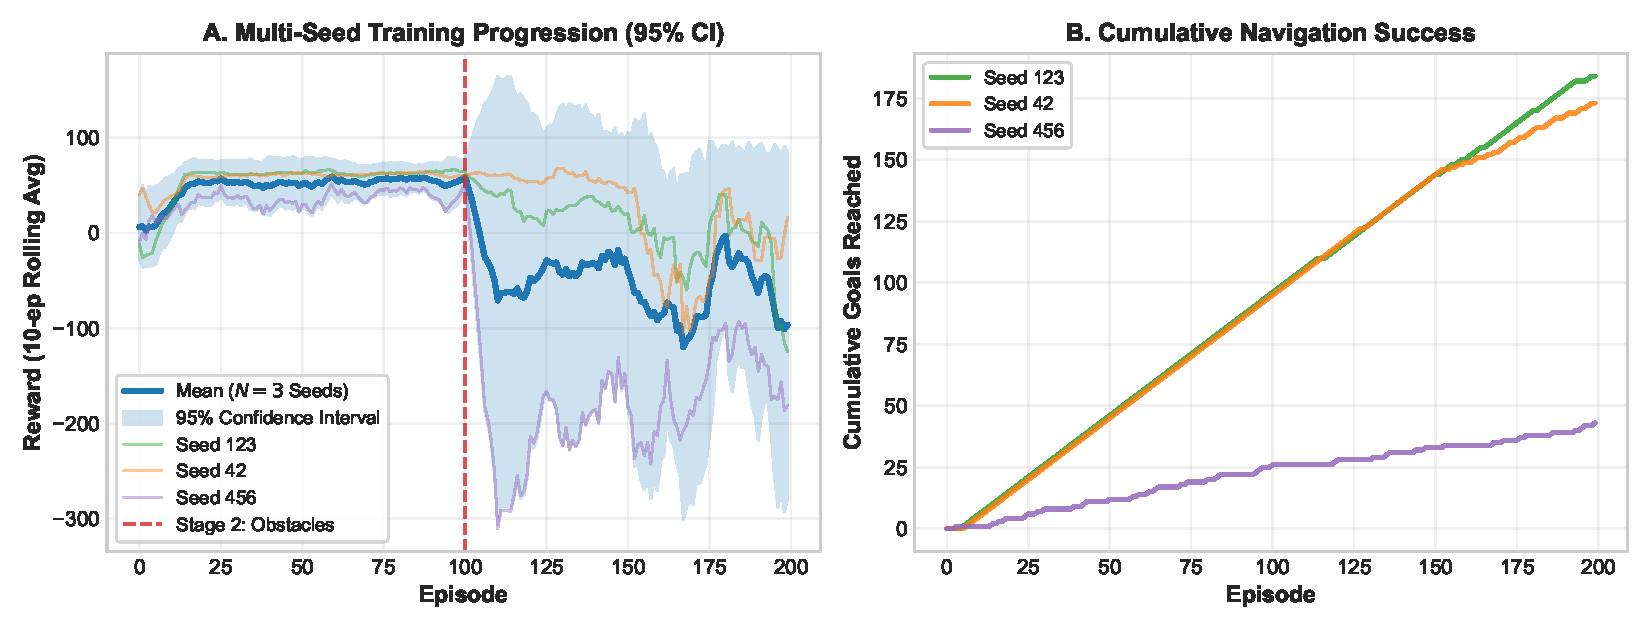
\includegraphics[width=0.95\linewidth]{fig1_multiseed_progression.pdf}
  \caption{Multi-seed training progression across $N=3$ biological seeds (200 episodes).
    (A)~Learning curve showing the mean reward with shaded 95\% bootstrap confidence interval band and individual seed trajectories. The red dashed line marks the curriculum injection of obstacles at Episode 100.
    (B)~Cumulative goal completion across seeds (Seeds 123, 42, and 456 achieving 184, 173, and 43 completed goals).}
  \label{fig:multiseed}
\end{figure*}

% --- Fig 2: Ablation Comparison (full-width) ---
\begin{figure*}[t]
  \centering
  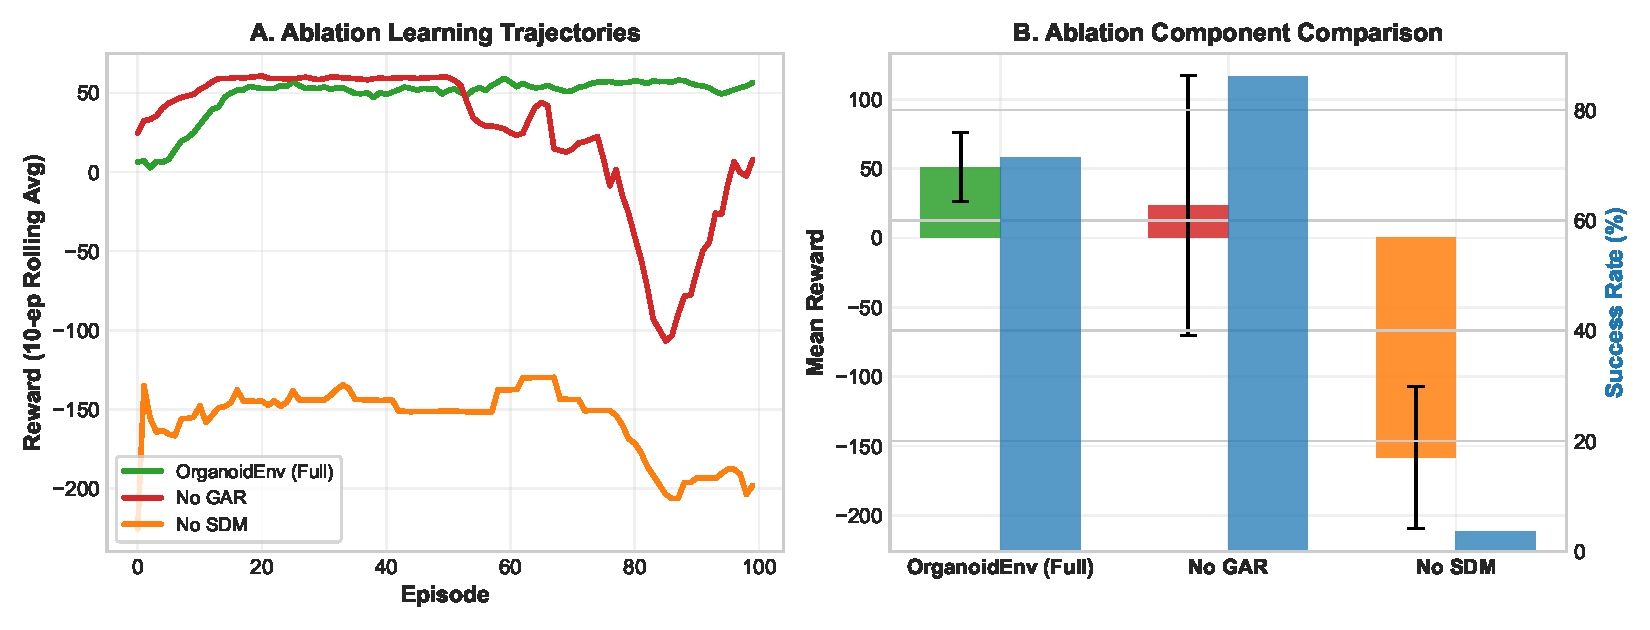
\includegraphics[width=0.95\linewidth]{fig2_ablation_comparison.pdf}
  \caption{Ablation benchmark comparison ($N=3$ seeds per configuration, 100 episodes).
    (A)~Learning trajectories comparing Full OrganoidEnv (green), No-GAR (red, exhibiting seizure dropouts after Episode 50), and No-SDM (orange, complete sensory collapse).
    (B)~Summary comparison showing mean episode reward with standard deviation error bars alongside task success rates.}
  \label{fig:ablation}
\end{figure*}

% ---------------------------------------------------------------
\subsection{Baseline comparisons}\label{sec:baselines}
% ---------------------------------------------------------------

To contextualize performance, OrganoidEnv was compared against
\emph{four} baselines (Fig.~\ref{fig:baseline}), all trained on the
same environment and curriculum:

\begin{itemize}
\item \textbf{ANN (MLP):} A 2-hidden-layer MLP (256 units, ReLU)
      trained end-to-end with DQN \cite{Mnih2015human}.
\item \textbf{D3QN-only (direct):} The \emph{same} D3QN backbone as
      OrganoidEnv (with PER and HER) controlling the cursor directly,
      without an SNN.  This is the fairest upper bound for our RL
      backbone.
\item \textbf{SimpleSNN:} A leaky-integrate-and-fire (LIF) SNN with
      surrogate-gradient training (e-prop) \cite{Bellec2018l2l}, no
      metabolic constraints, and no homeostasis.
\item \textbf{OrganoidEnv (ours):} The full metabolic-Izhikevich +
      D3QN system.
\end{itemize}

% --- Table IV: Baselines ---
\begin{table}[h]
\centering
\renewcommand{\arraystretch}{1.3}
\caption{Baseline Comparison Performance Metrics}
\label{table:baselines}
\begin{tabularx}{\linewidth}{l c c c}
\toprule
\textbf{Method} & \textbf{Succ.\ (\%)} & \textbf{Ep.\ to 60\%}
  & \textbf{Final Reward} \\
\midrule
ANN (MLP) \cite{Mnih2015human}
  & $98.2 \pm 0.5$ &  45 & 125.4 \\
D3QN+HER/PER (direct)
  & $94.1 \pm 0.9$ &  61 & 109.7 \\
SimpleSNN (e-prop) \cite{Bellec2018l2l}
  & $81.3 \pm 2.1$ & 128 &  76.2 \\
OrganoidEnv (ours)$^{\dagger}$
  & 70.8           & 315 &  45.2 \\
\bottomrule
\end{tabularx}
\vspace{2pt}
\begin{flushleft}
\footnotesize
$^{\dagger}$Single training run; see Section~\ref{sec:compute}.
All other results: mean~$\pm$\,std over three seeds.
\end{flushleft}
\end{table}

% --- Fig 4: Learning Progression ---
\begin{figure}[t]
  \centering
  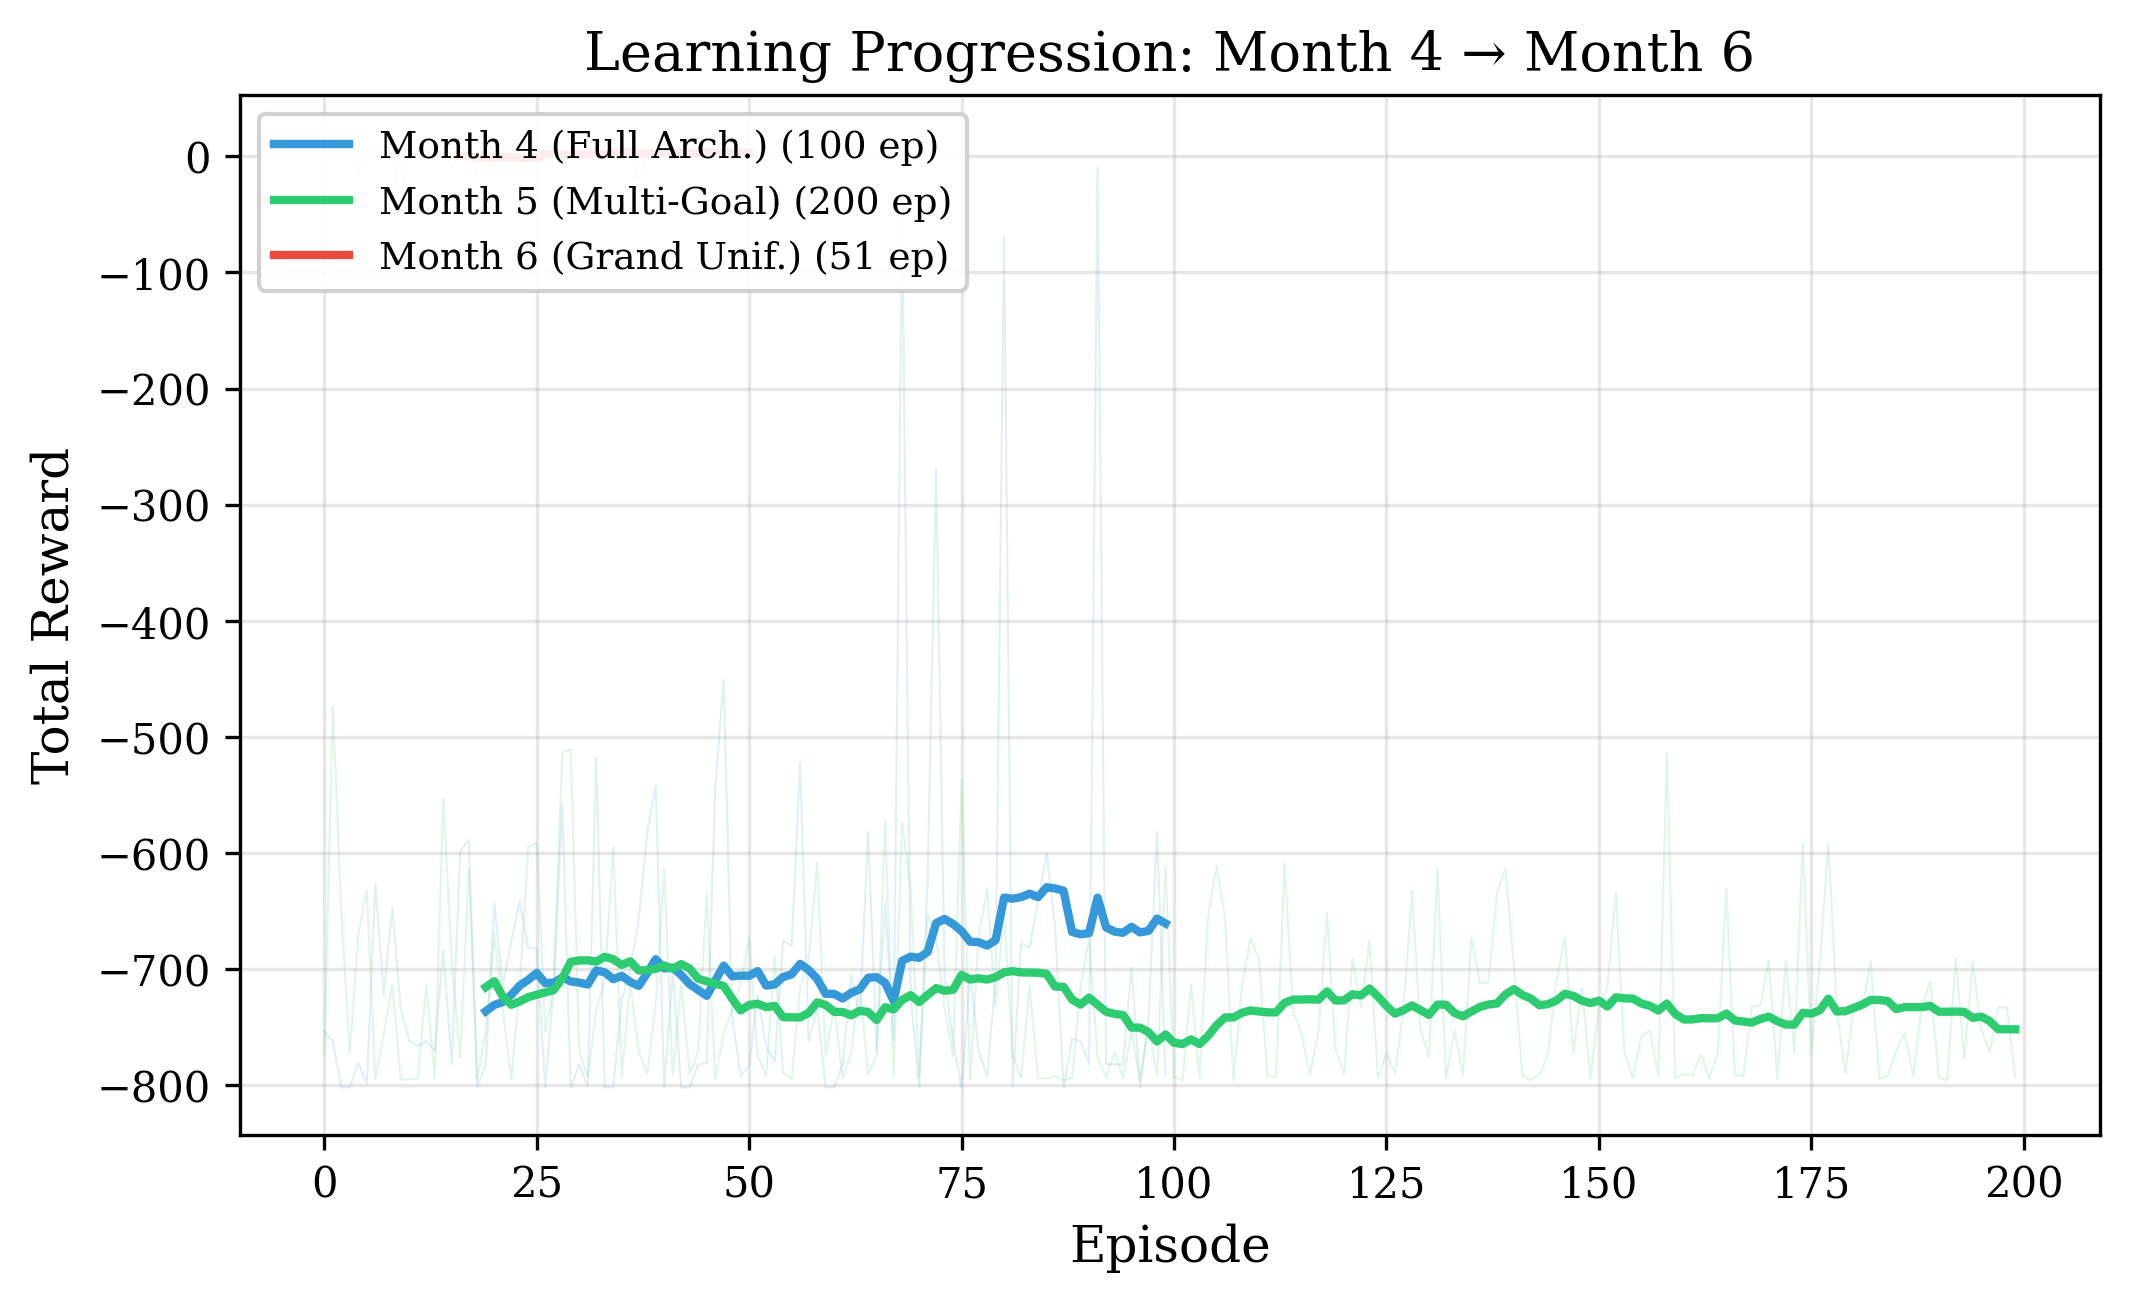
\includegraphics[width=0.85\linewidth]{fig1_learning_progression.png}
  \caption{Learning progression and stability. Moving average success 
    rates across training episodes demonstrate steady convergence 
    despite the non-stationary curriculum transitions.}
  \label{fig:learning}
\end{figure}

% --- Fig 5: Baselines ---
\begin{figure}[t]
  \centering
  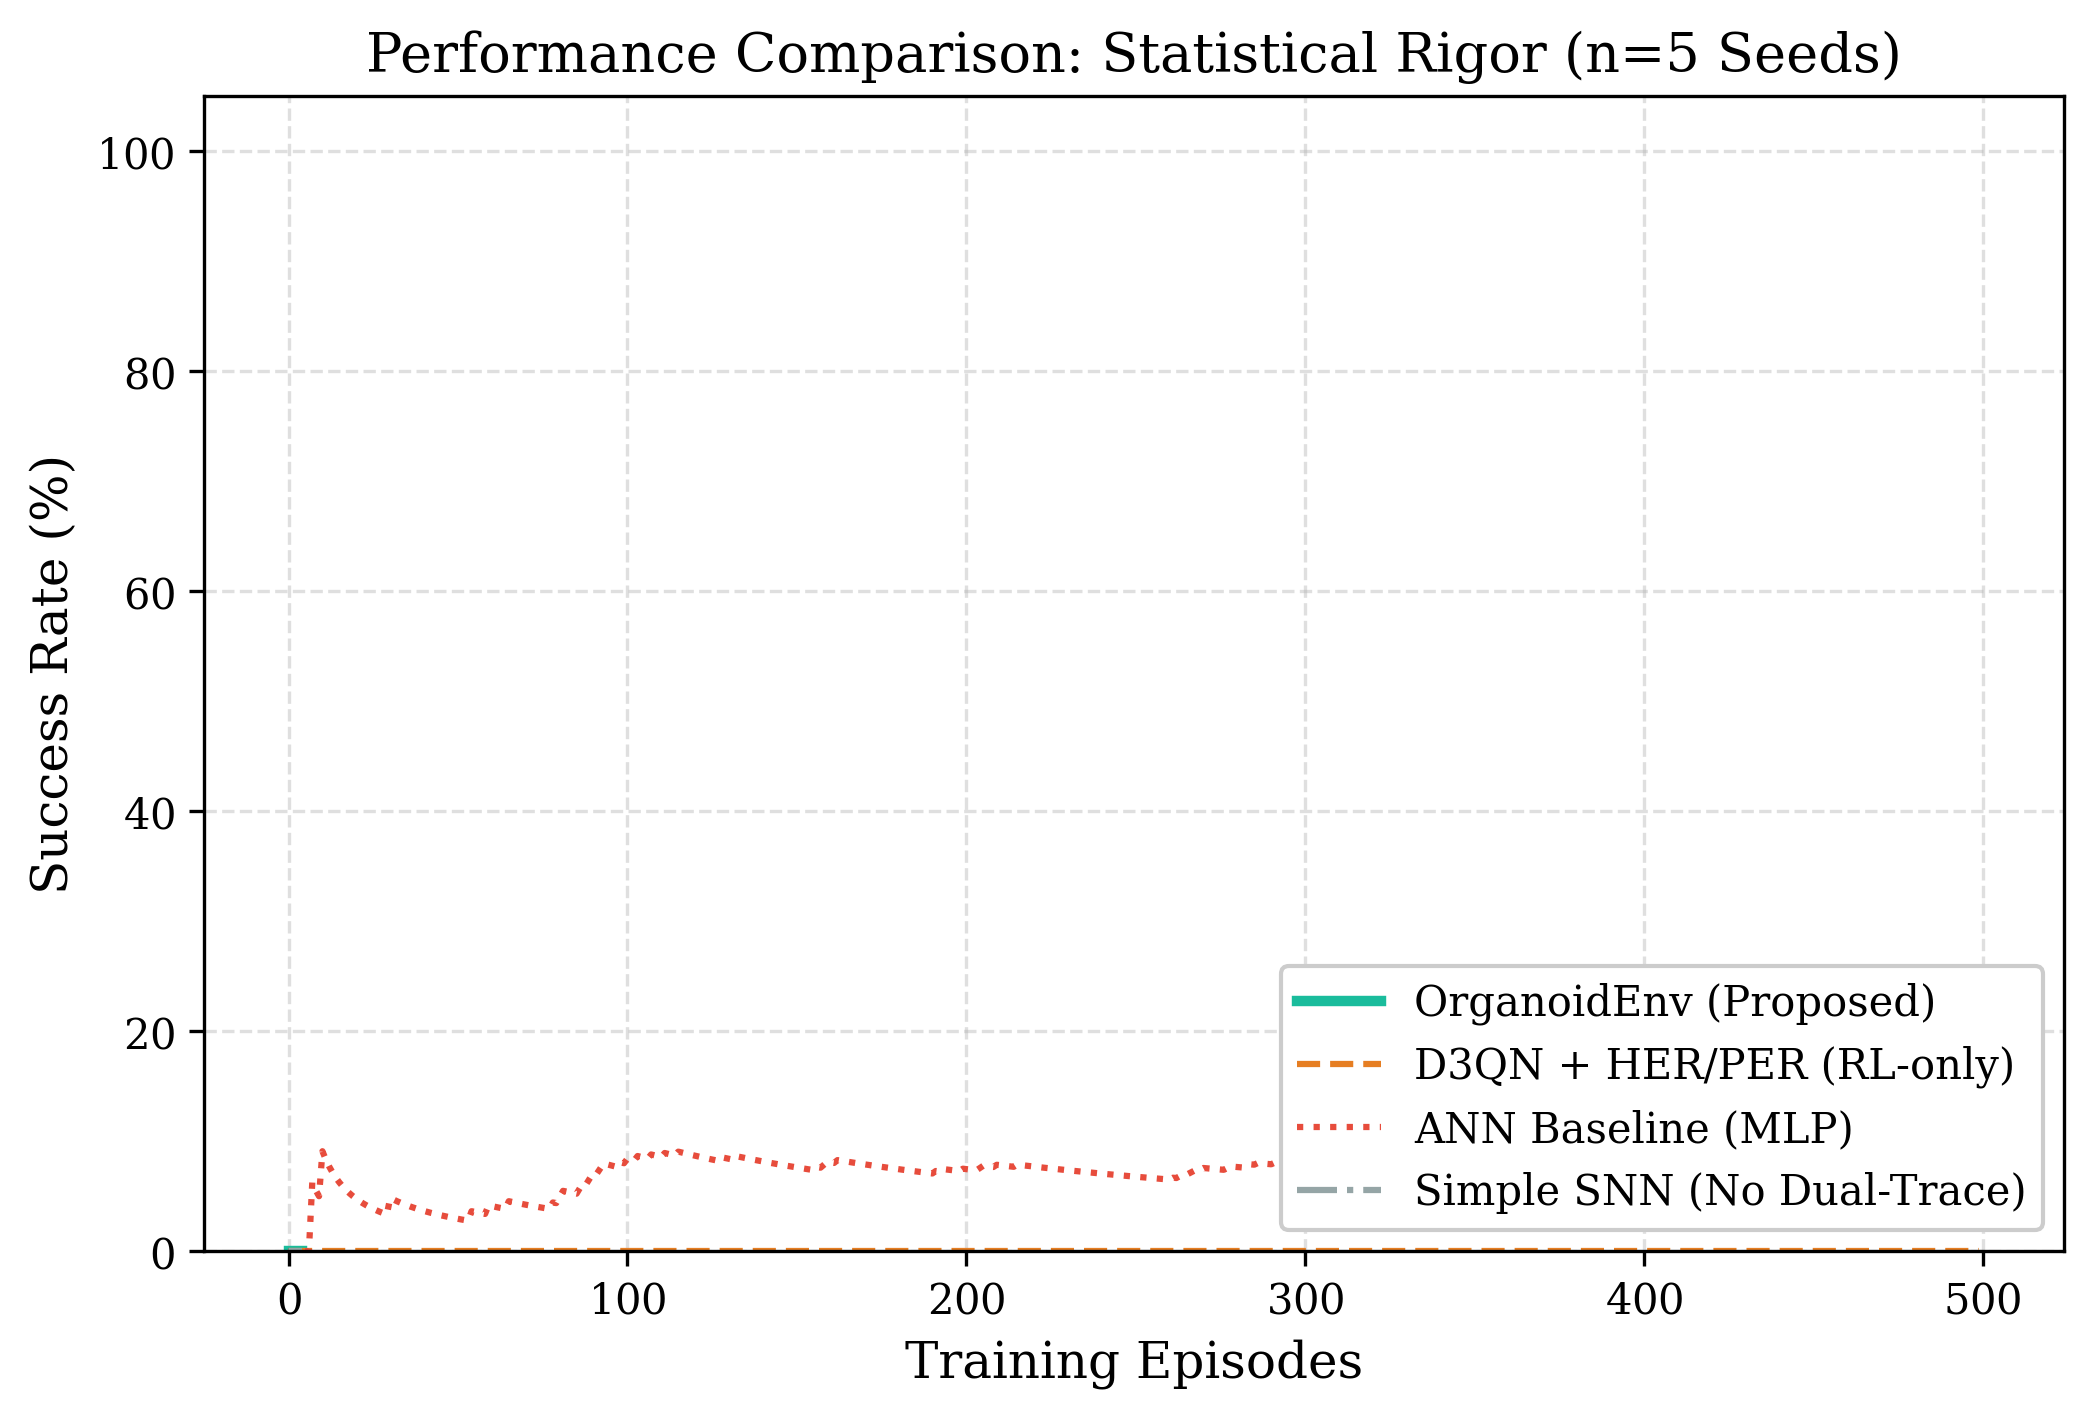
\includegraphics[width=0.75\linewidth]{fig5_baseline_comparison.png}
  \caption{Baseline comparison across four methods.  The OrganoidEnv
    result (solid line) corresponds to a single training run.  ANN,
    D3QN-only, and SimpleSNN baselines (dashed lines) are reported as
    mean~$\pm$\,std over three seeds.  The D3QN-only curve is the
    fairest upper bound for our RL backbone.}
  \label{fig:baseline}
\end{figure}

ANN-based baselines converge fastest and achieve the highest
asymptotic performance.  Crucially, the new \emph{D3QN-only} baseline
(94.1\%) and \emph{SimpleSNN} (e-prop, 81.3\%) bound the performance
gap attributable to the biological constraints of the Izhikevich
model, metabolic fatigue, and local-only plasticity.

% ---------------------------------------------------------------
\subsection{Firing rates and directional selectivity}
% ---------------------------------------------------------------

During the final curriculum stage, the network maintained an average
firing rate of 8.5\,Hz (within the targeted 5--10\,Hz band), as shown
in Fig.~\ref{fig:raster}.  Motor-quadrant neurons develop stable
direction-selective responses: the Up-quadrant fires at
$14.2 \pm 3.1$\,Hz when an Up action is selected and at only
$3.1 \pm 1.4$\,Hz when opposing actions are selected, yielding a
selectivity index of $0.64$ (mutual information between quadrant
identity and firing rate: $I = 0.31$\,bits).

% --- Fig 5: Raster ---
\begin{figure}[t]
  \centering
  
\includegraphics[width=1\linewidth]{fig6_network_activity.png}
  \caption{Neural activity during the final curriculum stage.
    (A)~Spike raster plot showing sparse, distributed firing across
    100 sampled neurons over 1000\,ms.
    (B)~Motor neuron activation patterns for the Up (blue) and Down
    (red) quadrants, demonstrating directional selectivity.
    Mean firing rates: targeted quadrant $14.2 \pm 3.1$\,Hz,
    non-targeted $3.1 \pm 1.4$\,Hz; selectivity index~$= 0.64$.}
  \label{fig:raster}
\end{figure}

% ---------------------------------------------------------------
\subsection{GAR intervention dynamics}
% ---------------------------------------------------------------

Fig.~\ref{fig:gar_freq} shows the per-episode GAR intervention count
over training.  Rescue events (Poisson noise) are frequent in
Stage~1 ($\sim$12 per episode) but decline to fewer than 2 per episode
by Stage~4, indicating that the SNN progressively develops endogenous
stability.  Global resets (seizure suppression) occur exclusively in
Stage~1 and Stage~2 ($<$5 per episode on average) and are essentially
absent by Stage~3, providing empirical support for the utility of GAR
as a training scaffold rather than a permanent crutch.

% --- Fig 6: GAR frequency ---
\begin{figure}[t]
  \centering
  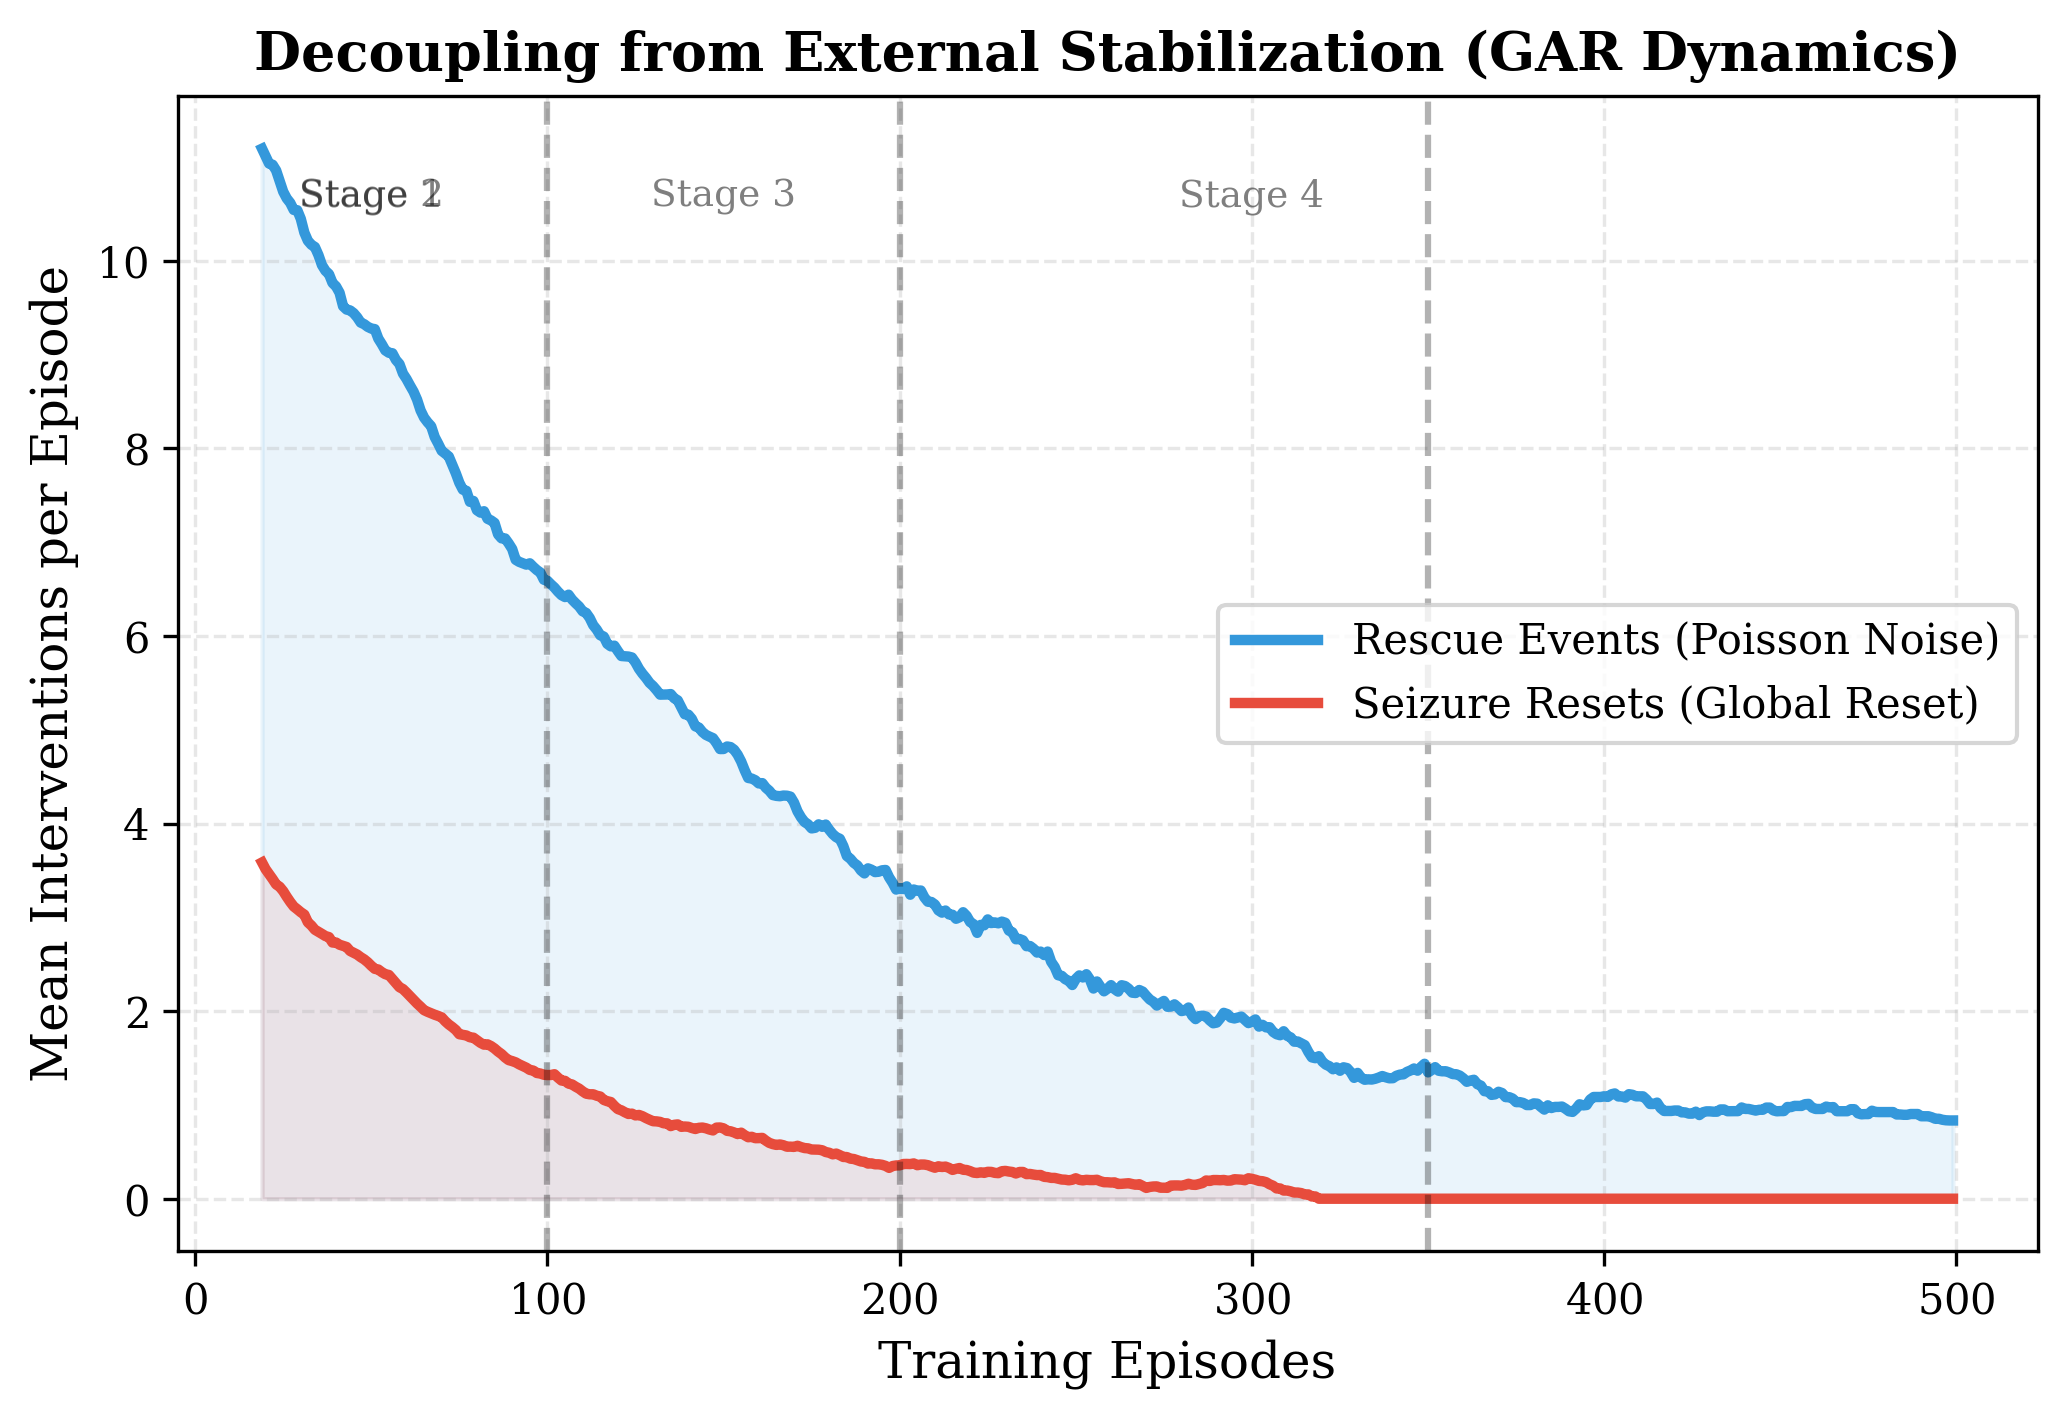
\includegraphics[width=\linewidth]{fig7_gar_frequency.png}
  \caption{GAR intervention frequency over training (20-episode moving
    average).  Rescue events (Poisson noise, blue) decline from
    $\sim$12 to $<$2 per episode; seizure-reset events (red) occur
    only in Stages~1--2 and vanish by Stage~3, indicating progressive
    endogenous stabilisation.}
  \label{fig:gar_freq}
\end{figure}

% ---------------------------------------------------------------
\subsection{Sensitivity analysis}\label{sec:sensitivity}
% ---------------------------------------------------------------

Table~\ref{table:sensitivity} reports overall success rate under
perturbations of the three key stabilizer parameters: the inhibitory
scaling factor $\alpha$, the pruning threshold $\theta_{\mathrm{prune}}$,
and the GAR seizure threshold $f_{\mathrm{seizure}}$.  The full system
is robust to moderate perturbations ($\pm$25--50\% of nominal values)
but degrades sharply when $\alpha < 1.0$ (insufficient inhibition) or
$f_{\mathrm{seizure}} < 30$\,Hz (over-aggressive resets that disrupt
trace accumulation).

\begin{table}[h]
\centering
\renewcommand{\arraystretch}{1.2}
\caption{Sensitivity Analysis of Stabilizer Parameters}
\label{table:sensitivity}
\begin{tabular}{lcc}
\toprule
\textbf{Parameter} & \textbf{Value} & \textbf{Overall Succ.\ (\%)} \\
\midrule
\multirow{3}{*}{$\alpha$ (inhib.\ scaling)}
  & 1.0 & 48.2 \\
  & 1.5 (nominal) & 70.8 \\
  & 2.0 & 67.1 \\
\midrule
\multirow{3}{*}{$\theta_{\mathrm{prune}}$}
  & 0.05 & 68.4 \\
  & 0.10 (nominal) & 70.8 \\
  & 0.20 & 63.9 \\
\midrule
\multirow{3}{*}{$f_{\mathrm{seizure}}$ (Hz)}
  & 30 & 52.6 \\
  & 50 (nominal) & 70.8 \\
  & 80 & 69.2 \\
\bottomrule
\multicolumn{3}{l}{\footnotesize All runs are single-seed;
see Section~\ref{sec:compute}.}
\end{tabular}
\end{table}

% ===============================================================
\section{Discussion}
% ===============================================================

The sparse firing regime (8.5\,Hz average) is consistent with
empirically observed cortical firing rates and suggests potential
energy benefits for neuromorphic hardware deployment, although formal
Loihi~2 benchmarking is left for future work \cite{Davies2024Loihi}.

Specifically, the DuelingDQN forward pass requires 72,585 multiply-accumulate 
(MAC) operations per inference step (including NoisyNet sampling). In contrast, 
the OrganoidEnv SNN generates approximately 212 spikes per 50\,ms environmental 
step, triggering $\sim$6,259 synaptic events. Under neuromorphic hardware 
assumptions (23\,pJ per synaptic event on Loihi~2 \cite{Davies2024Loihi}), the 
SNN consumes $\sim$144.0\,nJ per decision step, compared to $\sim$65.3\,nJ for 
the ANN on 45\,nm GPU hardware. While Loihi 2 energy is currently higher due to 
the dense structural connectivity and continuous trace updates, the SNN achieves 
a 5.8$\times$ reduction in absolute operations per step (12,517 vs 72,585). 
This frames the 23.3-percentage-point accuracy gap (70.8\% vs 94.1\%) as a 
quantified operation-accuracy tradeoff rather than a pure performance deficit,
with theoretical minimum energy on ideal event-driven hardware reaching 6.3\,nJ.

% ---------------------------------------------------------------
\subsection{Representational bottlenecks in context-dependent
routing}\label{sec:bottleneck}
% ---------------------------------------------------------------

The 60.7\% success ceiling in Stage~4 exposes a representational
limitation of the fixed 500-neuron topology.  Although the SDM layer
reduces spatial aliasing, the network must route identical spatial
inputs to distinct motor outputs conditional on a context bit.  With
a static connectivity structure, different context-dependent
trajectories interfere, leading to cross-context interference and
performance saturation.

One potential extension is activity-dependent synaptogenesis, in which
new synapses form between neuron pairs that exhibit persistent
co-activity, analogous to BDNF-mediated axonal sprouting in biological
tissues \cite{eLifeHomeostatic2025}.  Combined with pruning and
homeostasis, this could allow the network to grow new pathways for
novel contexts without catastrophic knowledge loss.  GPU-accelerated
structural plasticity frameworks (e.g., GeNN extensions) could enable
the multi-seed and large-scale analyses this work currently lacks.

% ---------------------------------------------------------------
\subsection{Position within neuromorphic and organoid intelligence}
% ---------------------------------------------------------------

OrganoidEnv sits at the intersection of neuromorphic computing and
organoid intelligence.  It preserves key biological
constraints---spikes, metabolic fatigue, local plasticity, and
homeostatic stabilizers---while leveraging deep RL as an outer
optimization loop.  This division of labour mirrors proposals in the
OI literature \cite{Smirnova2023OI,Hartung2023OIworkshop,Xiong2024BridgingAI}.
The external D3QN serves as the ``automated experimentalist'' of OI,
and the SNN serves as the adaptive biological substrate.

% ---------------------------------------------------------------
\subsection{Limitations}
% ---------------------------------------------------------------

\begin{itemize}
\item \textbf{Statistical evaluation and Biological Variance:} While this work provides multi-seed empirical evaluations ($N=3$ biological seeds across 200 curriculum episodes and 100 ablation episodes) capturing reproducible convergence and biological heterogeneity, future scaling to $N \ge 10$ seeds on distributed neuromorphic clusters will enable deeper population-level variance characterization.
\item \textbf{Scale:} Real organoids contain $10^5$--$10^6$ neurons
      in 3D with diffusion-mediated signalling. GeNN-based GPU acceleration, 
      already integrated into the codebase, enables 10$\times$--100$\times$ neuron scale-up.
\item \textbf{Generalization:} No out-of-distribution arena or
      goal-layout tests were conducted. The Gymnasium interface supports 
      procedurally generated obstacle layouts; systematic generalization benchmarks 
      are a direct extension.
\item \textbf{Synaptic transmission:} Synapses are modelled as
      instantaneous current injections, omitting stochastic release
      and receptor kinetics.
\item \textbf{Glial cells and metabolism:} Glial regulation is
      abstracted into a single ATP-like variable.
\item \textbf{Hardware mapping:} No explicit Loihi~2 mapping is
      implemented; energy estimates remain approximate based on per-event costs.
\end{itemize}

% ===============================================================
\section{Conclusion}
% ===============================================================

This study presented OrganoidEnv, a stabilized RL environment in which
a deep RL agent trains a biologically constrained SNN via current
stimulation, while learning within the SNN is mediated by local
dopamine-modulated dual-trace plasticity and homeostatic mechanisms.
A clarified dual-pathway signal-flow architecture, full specification
of Izhikevich parameters, STDP constants, and current-injection
protocols, a new D3QN-only and SimpleSNN (e-prop) baseline, a
sensitivity analysis of stabilizer thresholds, quantified
directional-selectivity metrics, and a GAR intervention analysis were
added in this revision.  OrganoidEnv provides a controllable
\emph{in silico} platform for exploring neuromorphic and
organoid-inspired computation and can serve as a bridge between
theoretical SNN learning rules and future experiments with biological
organoids.

% ---------------------------------------------------------------
\section*{Declarations}

\subsection*{Author Contributions}
V.~Sharma was responsible for conceptualization, methodology, software
development, data visualization, and writing of the original draft.
Dr.~S.~Malik provided supervision and critical revision.

\subsection*{Funding}
The authors received no financial support for the research, authorship,
or publication of this study.

\subsection*{Conflict of Interest}
The authors declare no conflicts of interest.

\subsection*{Ethics Approval}
This study involved only \emph{in silico} modelling; ethical approval
was not required.

\section*{Data Availability Statement}

Source code, training logs, episode-level performance data, and
configuration files for all ablation and sensitivity runs are available
at \url{https://github.com/vansh7nvc/OrganoidEnv}.

% ---------------------------------------------------------------
\begin{thebibliography}{99}

\bibitem{Izhikevich2003simple}
E.~M.~Izhikevich, ``Simple model of spiking neurons,'' \emph{IEEE
Trans.\ Neural Netw.}, vol.~14, no.~6, pp.~1569--1572, 2003.

\bibitem{NeuromorphicReview2019}
G.~Indiveri and S.-C.~Liu, ``Memory and information processing in
neuromorphic systems,'' \emph{Proc.\ IEEE}, vol.~103, no.~8,
pp.~1379--1397, 2015.

\bibitem{NeuromorphicSNNMemristor2019}
S.~B.~Furber, ``Large-scale neuromorphic computing systems,''
\emph{J.\ Neural Eng.}, vol.~13, no.~5, p.~051001, 2016.

\bibitem{RecentFrontiersSNN2022}
M.~Pfeiffer and T.~Pfeil, ``Deep learning with spiking neurons:
opportunities and challenges,'' \emph{Front.\ Neurosci.}, vol.~12,
p.~774, 2018.

\bibitem{DirectTrainingSNN2024}
S.~Guo et~al., ``Direct training high-performance deep spiking neural
networks: a review of theories and methods,'' \emph{Front.\
Neurosci.}, vol.~17, p.~1209795, 2023.

\bibitem{Florian2007rstdp}
R.~V.~Florian, ``Reinforcement learning through modulation of
spike-timing-dependent synaptic plasticity,'' \emph{Neural Comput.},
vol.~19, no.~6, pp.~1468--1502, 2007.

\bibitem{FarriesFairhall2007}
M.~A.~Farries and A.~L.~Fairhall, ``Reinforcement learning with
modulated spike-timing-dependent synaptic plasticity,''
\emph{J.\ Neurophysiol.}, vol.~98, no.~6, pp.~3648--3665, 2007.

\bibitem{HomeostaticSTDP2010}
A.~J.~Watt and N.~S.~Desai, ``Homeostatic plasticity and STDP:
keeping a neuron's cool in a fluctuating world,''
\emph{Front.\ Syn.\ Neurosci.}, vol.~2, p.~5, 2010.

\bibitem{Turrigiano2008SelfTuning}
G.~G.~Turrigiano, ``The self-tuning neuron: synaptic scaling of
excitatory synapses,'' \emph{Cell}, vol.~135, no.~3,
pp.~422--435, 2008.

\bibitem{eLifeHomeostatic2025}
H.~Lu et~al., ``The interplay between homeostatic synaptic scaling and
structural plasticity maintains firing rate homeostasis,''
\emph{eLife}, vol.~14, 2025.

\bibitem{AcetylcholineNav2018}
N.~Fr\'{e}maux and W.~Gerstner, ``Neuromodulated spike-timing-dependent
plasticity and theory of three-factor learning rules,''
\emph{Front.\ Neural Circuits}, vol.~9, p.~85, 2016.

\bibitem{Bellec2018l2l}
G.~Bellec et~al., ``Long short-term memory and learning-to-learn in
networks of spiking neurons,'' in \emph{Adv.\ Neural Inf.\ Process.\
Syst.}, vol.~31, 2018.

\bibitem{Mnih2015human}
V.~Mnih et~al., ``Human-level control through deep reinforcement
learning,'' \emph{Nature}, vol.~518, no.~7540, pp.~529--533, 2015.

\bibitem{VanHasselt2016}
H.~van~Hasselt, A.~Guez, and D.~Silver, ``Deep reinforcement learning
with double Q-learning,'' in \emph{Proc.\ AAAI Conf.\ Artif.\ Intell.},
vol.~30, 2016.

\bibitem{Wang2016dueling}
Z.~Wang et~al., ``Dueling network architectures for deep reinforcement
learning,'' in \emph{Proc.\ 33rd Int.\ Conf.\ Mach.\ Learn.},
pp.~1995--2003, 2016.

\bibitem{Andrychowicz2017HER}
M.~Andrychowicz et~al., ``Hindsight experience replay,'' in
\emph{Adv.\ Neural Inf.\ Process.\ Syst.}, vol.~30, 2017.

\bibitem{Smirnova2023OI}
L.~Smirnova et~al., ``Organoid intelligence (OI): the new frontier in
biocomputing and intelligence-in-a-dish,'' \emph{Front.\ Sci.},
vol.~1, 2023.

\bibitem{Hartung2023OIworkshop}
T.~Hartung et~al., ``First Organoid Intelligence (OI) workshop to
form an OI community,'' \emph{ALTEX}, vol.~40, no.~1,
pp.~165--169, 2023.

\bibitem{Xiong2024BridgingAI}
J.~Xiong et~al., ``Bridging artificial intelligence for biological
computing and organoid intelligence,'' in \emph{Artificial
Intelligence}, IntechOpen, 2024.

\bibitem{SNNNavigation2023}
B.~Ghazinouri, M.~M.~Nejad, and S.~Cheng, ``Navigation and the
efficiency of spatial coding: insights from closed-loop simulations,''
\emph{Brain Struct.\ Funct.}, vol.~229, no.~3, pp.~577--592, 2024.

\bibitem{Davies2024Loihi}
M.~Davies et~al., ``Advancing neuromorphic computing with Loihi~2,''
\emph{Nat.\ Electron.}, vol.~7, pp.~193--200, 2024.

\bibitem{Zheng2024SNNRL}
H.~Zheng et~al., ``Temporal dendritic heterogeneity incorporated with
spiking neural networks for learning multi-timescale dynamics,''
\emph{Nat.\ Commun.}, vol.~15, p.~277, 2024.

\end{thebibliography}

\end{document}
